% !TeX root = ../main.tex
% Add the above to each chapter to make compiling the PDF easier in some editors.

\chapter{Introduction}\label{chapter:introduction}

WebAssembly is enabling new experiences on the web and could become a widely used universal bytecode outside of browsers as well. After bringing near-native performance to the web, new use-cases for WebAssembly emerge in the embedded market. In late 2019 the first runtimes for WebAssembly on microcontrollers became publicly available and made it an interesting technology for the IoT market. As defined by Gartner \autocite{gartner_internet_nodate}
\begin{displayquote}
    The Internet of Things (IoT) is the network of physical objects that contain embedded technology to communicate and sense or interact with their internal states or the external environment.
\end{displayquote}

Spending on the Internet of Things is prognosed to increase from \SI{646}[\$]{B} in 2018 to \SI{1100}[\$]{B} in 2023 \autocite{idc_prognosis_2019}. As visible in figure \ref{fig:iot_connections} the number of connected IoT devices is rising steadily as well. This very big market \textquote{is moving beyond the hype}\autocite{gartner_internet_nodate-1} and will continue to see a lot of innovation and interest.

\begin{figure}[h]
    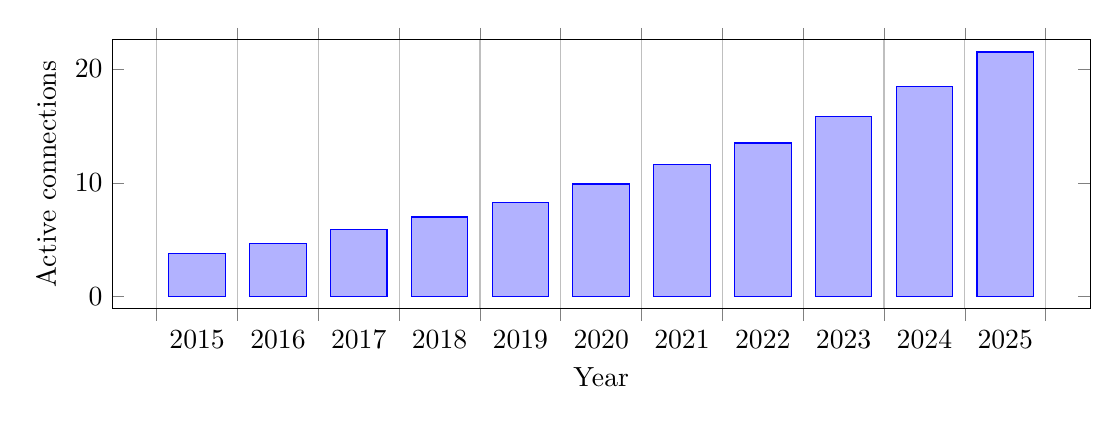
\begin{tikzpicture}
        \begin{axis}[
                x tick label style={
                    /pgf/number format/1000 sep=},
                ylabel=Active connections,
                xlabel=Year,
                width=14cm,
                height=5cm,
                enlargelimits=0.05,
                ybar interval=0.7,
            ]
            \addplot coordinates {(2015,3.8) (2016,4.7) (2017,5.9) (2018,7) (2019,8.3) (2020,9.9) (2021,11.6) (2022,13.5) (2023,15.8) (2024,18.5) (2025,21.5) (2026,0)};
        \end{axis}
    \end{tikzpicture}
    \caption{IoT active device connections in billions \autocite{iot_analytics_internet_2018}}
    \label{fig:iot_connections}
\end{figure}

If WebAssembly can be used on IoT devices, it opens the programming of embedded devices up for new deployment models and new languages that were previously not supported. Being a universal bytecode that is optimized for being transmitted over the network, it can be used to send the same program to many different devices over the air.

There is not much research available that concerns the usage of WebAssembly in embedded devices or the ESP32 specifically. Most of the research is currently focused on the applications inside the browser. In this thesis, we want to layout a method to assess the feasibility of running WebAssembly and explore its drawbacks and advantages. Before we explain our approach, we will give some background on the essential parts of the work. 

\paragraph{Microcontrollers}
Meant for executing specific tasks, microcontrollers are small computers with minimal resources. They are designed with the aim to have just enough resources while keeping costs low. A popular system on a chip in this class is the ESP32 family. They are very affordable and can be used from experimentation and prototyping to production products. Their connectivity options and CPU performance makes them a great fit for IoT devices. We will test running WebAssembly on the ESP32 in this thesis, which uses the realtime operating system FreeRTOS.

\paragraph{WebAssembly}
Since its beginning with static pages, the web has evolved to become a universal platform for applications, available on many different devices. However, even though browser engines have made significant progress at optimizing JavaScript, the only natively supported language on the web, the performance is still not reliable and depends on the optimizations deployed by the browser engine. To solve this problem, WebAssembly was created. It is a new, low-level bytecode format that allows running optimized code on browsers at near-native speeds. Being adopted by all major browser vendors, it is now almost universally available \autocite{deveria_can_nodate}.

However, since WebAssembly has no explicit dependencies on the web platform, its attributes such as portability, safety, and speed, making it very useful outside of the browser too. Runtimes meant to be used on embedded devices have become available recently and might open exciting new options for programming a microcontroller.

\section*{Assessing WebAssembly}

In order to assess the current state of WebAssembly on the ESP32, we found a runtime, WASM3, which has support for the ESP32 running FreeRTOS. While other runtimes are available already, most of them only target desktop PCs. The only other runtime for embedded use, the WebAssembly micro runtime, does not support the ESP32 operating system. WASM3 also achieves the best execution speeds amongst WebAssembly runtimes in benchmarks \autocite{shymanskyy_wasm3_2020}.

The comparison we are interested in is between the execution of code compiled to WebAssembly and compiled to native code. For this, we designed a collection of Workloads\footnote{All tests can be accessed at \url{https://github.com/Isigiel/bsc-thesis/tree/master/code/platforms}} that are inspired by real-world applications. We ran those tests as WebAssembly and native code and measured the different behavior to gain more insight into the drawbacks and advantages of running WebAssembly.

After running the test and interpreting results, we will draw some learnings from our measurements and research that can help developers when considering it for a new IoT project. Apart from that, all tests are meant to be reproducible on other hardware platforms or with other engines once they are released to compare the performance and asses WebAssembly in other setups. If a new runtime for embedded devices is published, they can be rerun with minor changes to have an immediate comparison.